\section{Evaluation}
\label{s:results}

Adding computation to the network increases latency and consumes memory. Our
evaluation demonstrates that by applying our techniques we are able to see
significant performance boosts in terms of overall throughput, and latency for
existing systems. We discuss the memory implications and show that systems
performance can be significantly improved by replacing compare and swap
operations with writes.

\subsection{Testbed}

Our testbed consists of five machines: a Clover memory server, metadata server,
and two Clover clients; the last machine hosts {\sword}. Physically, the
machines are identical: each is equipped with two Intel Xeon E5-2640 CPUs and
256 GB of main memory evenly spread across the NUMA domains. Each server is
equipped with a Mellanox ConnectX-5 100-Gbps NIC installed in a 16x PCIe slot,
all of which are connected to a 100-Gbps Mellanox Onyx Switch. All Clover
servers are configured with default routing settings: clients send directly to
the metadata and data servers. We install OpenFlow rules on the Onyx switch to
redirect the Clover RDMA traffic to \sword; \textbf{\todo{XXX:}}
Figure~\ref{f:testbed} shows the layout of our testbed.

\subsection{YCSB Benchmarks}

\begin{figure*}
    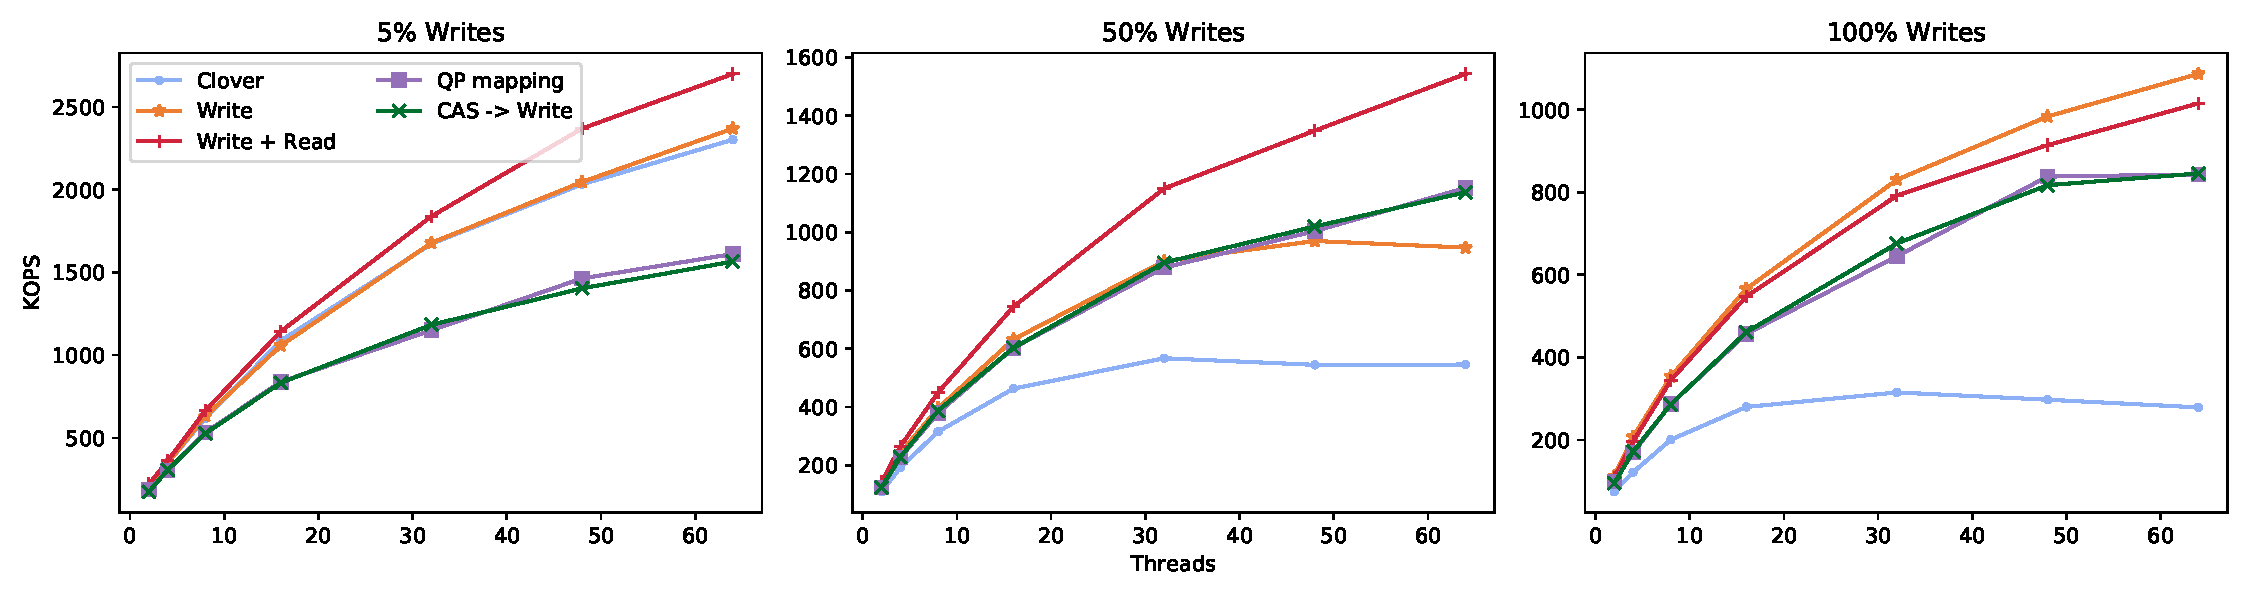
\includegraphics[width=1.0\textwidth]{fig/full_system_performance.pdf}

    \caption{{Performance of \sword techniques relative to clover on YCSB
    benchmarks. The percentage of workload writes increases from left to
    right.}}

    \label{fig:full_system_performance}
\end{figure*}

The YCSB benchmark consists of varying read and write workloads which have been
shown to emulate many common data center operations~\cite{ycsb}. We show a
breakdown of our techniques, mainly read and write caching, QP mapping, and
atomic replacement with respect to their effect to system performance on two
YCSB benchmarks. We choose YCSB-B (95\% read and 5\% write) as our baseline, and
YCSB-A (50\% read and 50\% write) to demonstrate how our algorithm performs
under high contention.  We also show the performance boosts obtained while
running a 100\% write workload which is intended to emulate other programmatic
workloads which are update heavy.

Figure~\ref{fig:full_system_performance} shows the relative performance gains
from each of \sword's techniques. At 5\% read the performance improvement is
minimal in terms of write steering as the vast majority of writes succeed on
their first try. Individual writes can lead to many stale reads immediately
after which leads write steering to offer a 1.17x throughput improvement.
Applying QP mapping to the read majorly case adds too much computational
overhead to give a benefit when writes are low, and only a few compare and swap
operations exist. 

At 50\% writes, clover is sufficiently outside of it's operational domain, that
at 64 threads, over half of all write operations fail. Here applying write
steering gives 1.73x at 64 cores. Write steering only is not sufficient at this
workload. While all writes succeed they can easily outstrip reads causing the
majority of them to fail (above 50\% at 64 threads).
Figure~\ref{fig:tail_latency} shows the effect of only applying write steering
to read latencies. Applying both read and write steering yields a 2.82x
throughput improvement as nearly all operations succeed. This workload leads to
enough common case failures that performance overhead of performing QP mapping
still yields a performance boost.

Write only workloads are antagonistic for Clover. Applying write steering and
read steering yield 3.89x and 3.63x throughput improvements respectively. No
reads occur so read steering is pure overhead.



%%\todo{real takeaways}

% \subsection{Memory Utilization}
% Our techniques give a performance boost at the cost of in network memory. We
% took special care to design our algorithms so that they could 1) use only a
% small amount of network memory, 2) be scalable depending on the resources
% available. We show how our performance varies as a function of the available in
% network state.

% As seen in Figure~\ref{fig:cache} our write caching is able to provide a
% significant performance boost while only using a small number of cached
% addresses. In the following experiment we show the maximum performance boost we
% can provide as a function of the available in network memory. Specifically in
% the case of read and write caching this means shrinking the size of the
% available cache. In terms of QP mapping it restricts the number of connections
% which can have their connections mapped. Unmapped connections must use atomic
% operations for their requests to succeed.

% \begin{figure}
%     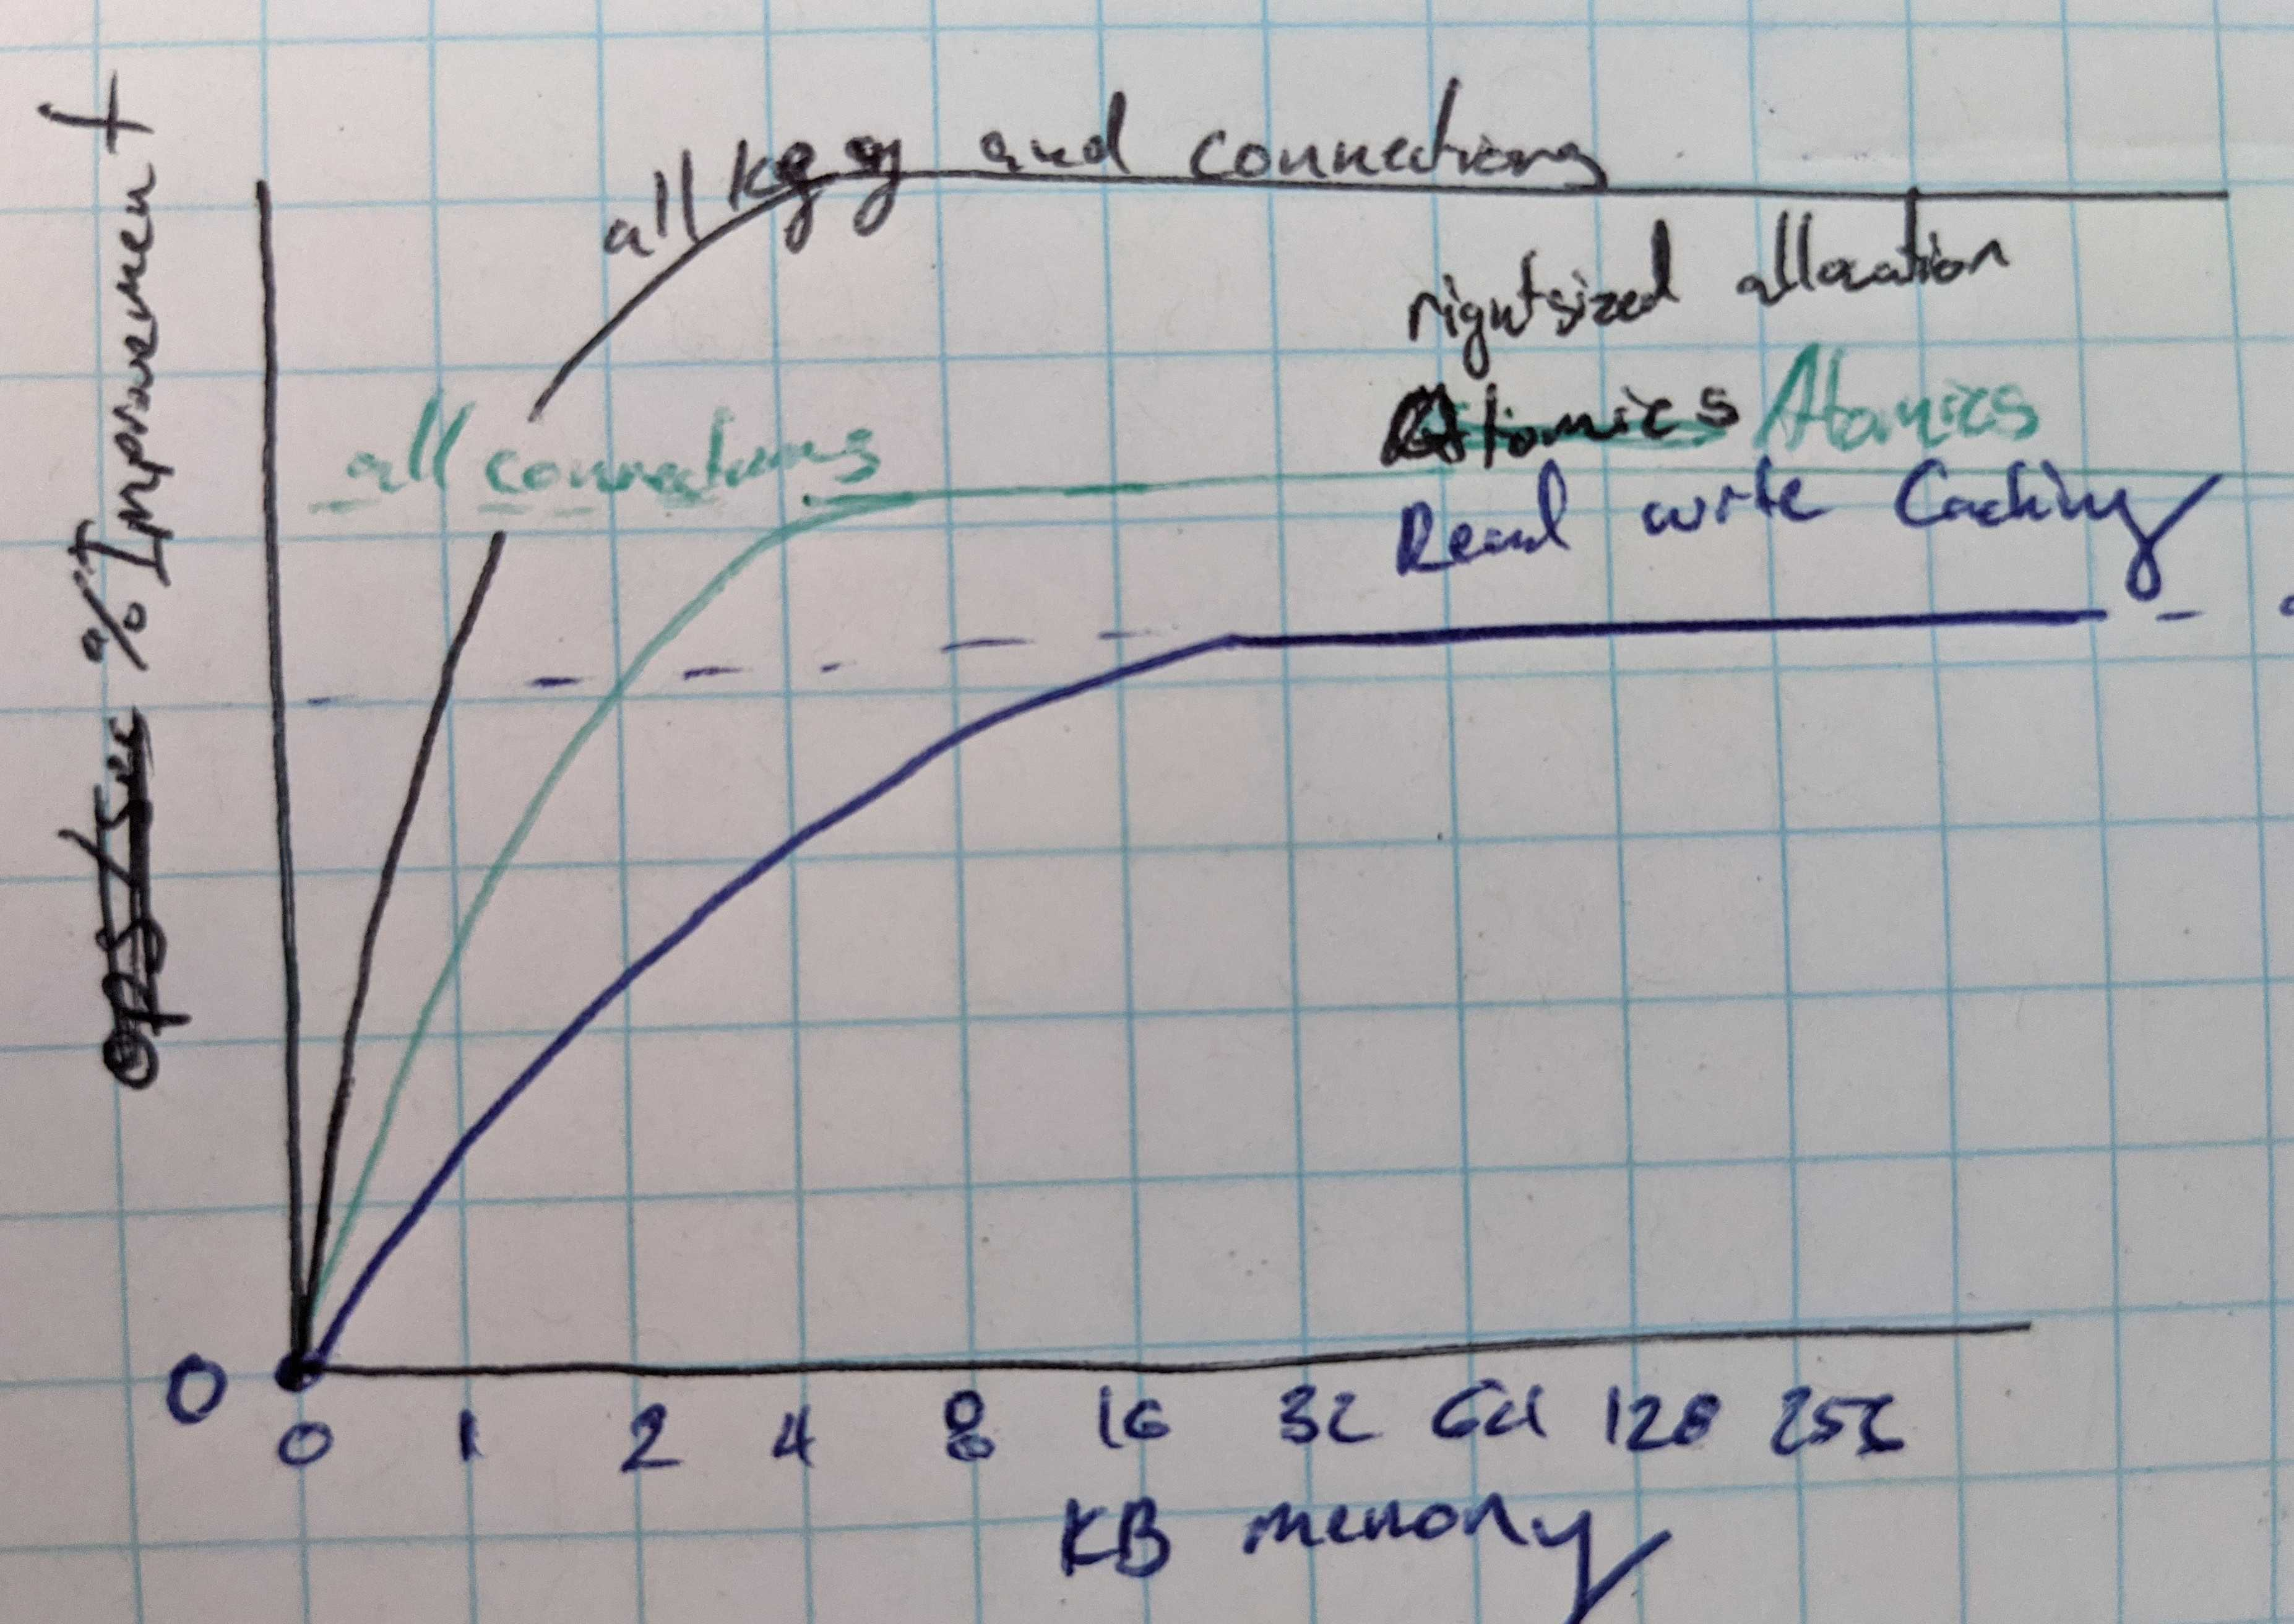
\includegraphics[width=0.45\textwidth]{fig/memory_util.jpg}
%     \caption{{Relative performance improvement of our techniques with restricted amounts of memory. Here a rightsized allocation implies that for the given number of connections we could support, all requests were mapped and reads and writes were cached.}}
%     \label{fig:memory_util}
% \end{figure}
%%\todo{say something real about the the memory utilization takeaways}


\subsection{Bandwidth Reduction}

Placing memory operations in band with regular network traffic can be
problematic as applications remote memory usage has the potential to vary
dramatically per application. When under contention resources require additional
packets which inflate the bandwidth necessary for a single operation. Our in
network steering algorithm, removes the need for operations to retry.
Figure~\ref{fig:bandwidth_reduction} shows the percentage of bandwidth reduced
per operation when resources are contested under different workloads.

\begin{figure}
    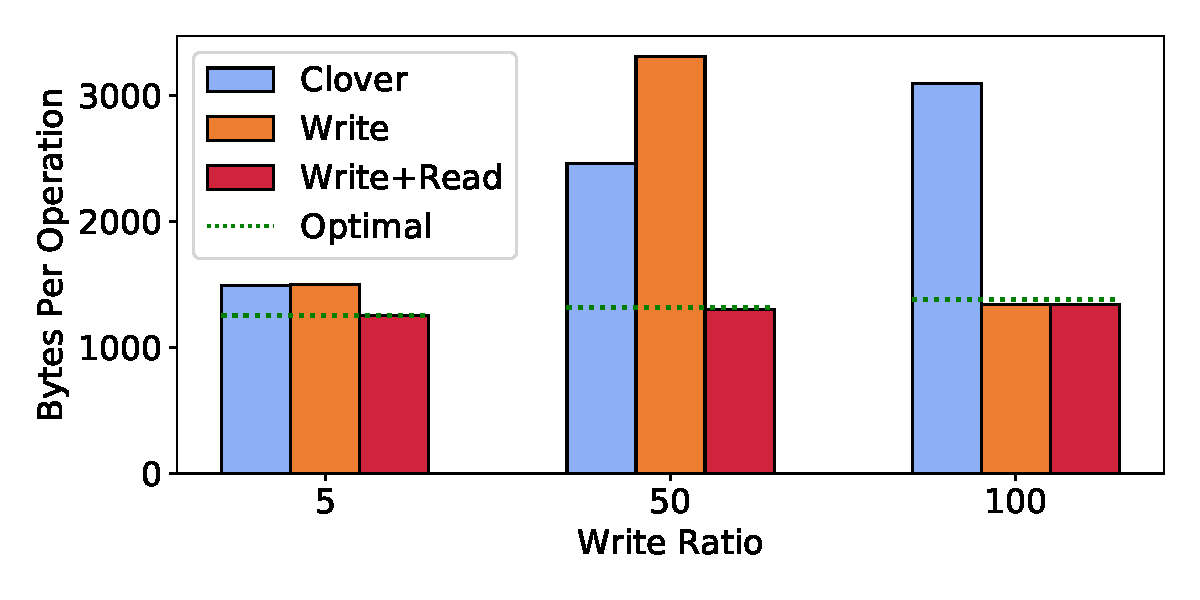
\includegraphics[width=0.5\textwidth]{fig/bandwidth_reduction.pdf}
    \caption{{Bandwidth reduction when in network steering is applied}}
    \label{fig:bandwidth_reduction}
\end{figure}

We calculate the optimal cost of each clover operation by averaging the cost of
a successful operation in bytes for both reads, and for writes. We get the
average measure by multiplying the cost of a read, and write by a coefficient
for the workloads write percentage. Each write consists of an RDMA write
followed by a CAS, along with the responses for each message. A read consists of
a read and read response, as well as an opportunistic read made asynchronously
with the main read to fetch the latests position of the tail A read consists of
a read and read response, as well as an opportunistic read made asynchronously
with the main read to fetch the latests position of the tail in case the read
fails. This second operation executes opportunistically (around 99 percent of
all reads), however sometimes it is omitted leading to a small over approximation
in our optimal estimate. 


Figure~\ref{fig:bandwidth_reduction} Show the cost of each operation in terms of
bandwidth across write workloads. We calculate the value for each technique by
summing the total bandwidth across a run, and dividing by the total number of
operations. In each case Read+Write operates near optimal. Write steering alone
causes significant inflation in the cost of operations at 50\% write as many
operations fail. Clovers bandwidth inflates by 1.8x at 50\% and 2.24x at 100\%
writes.


\subsection{Tail Latency}

\begin{figure*}
    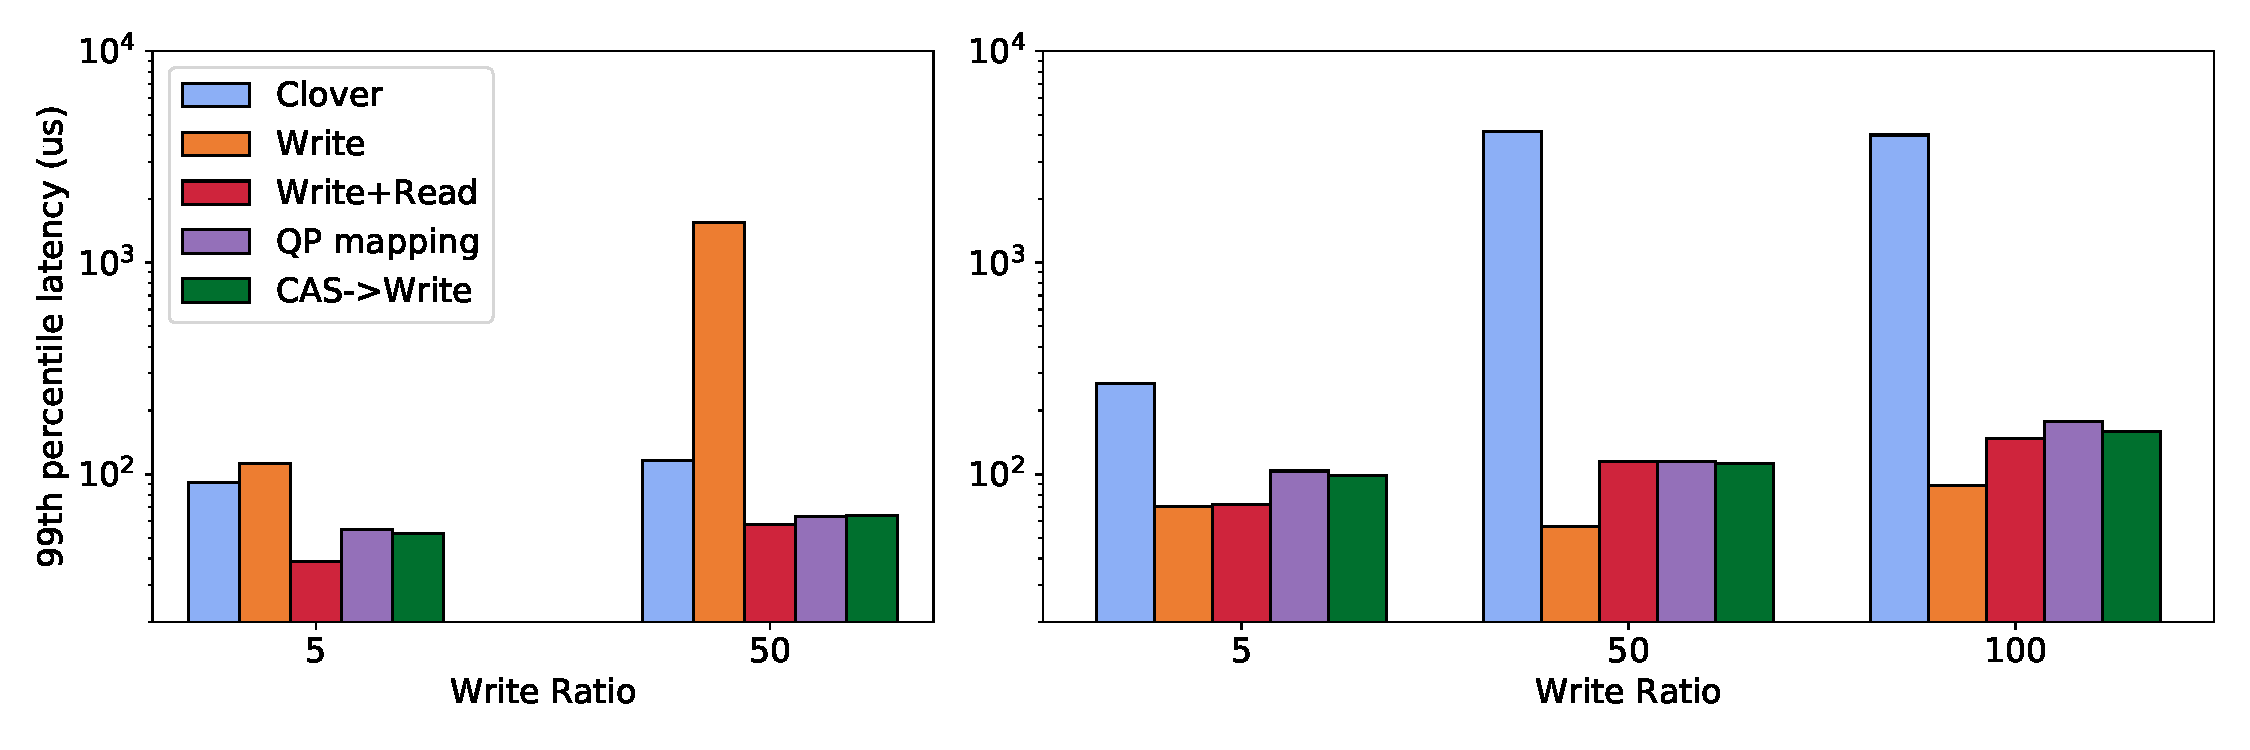
\includegraphics[width=1.0\textwidth]{fig/99th_latency.pdf}

    \caption{Left: Read tail latencies 99th percentile. Right: Write latencies.
    Each measure taken on a zipf distribution of requests with 64 clients. Note that the y axis is log scale}

    \label{fig:tail_latency}
\end{figure*}

\subsection{CAS to write performance}

\begin{figure}
    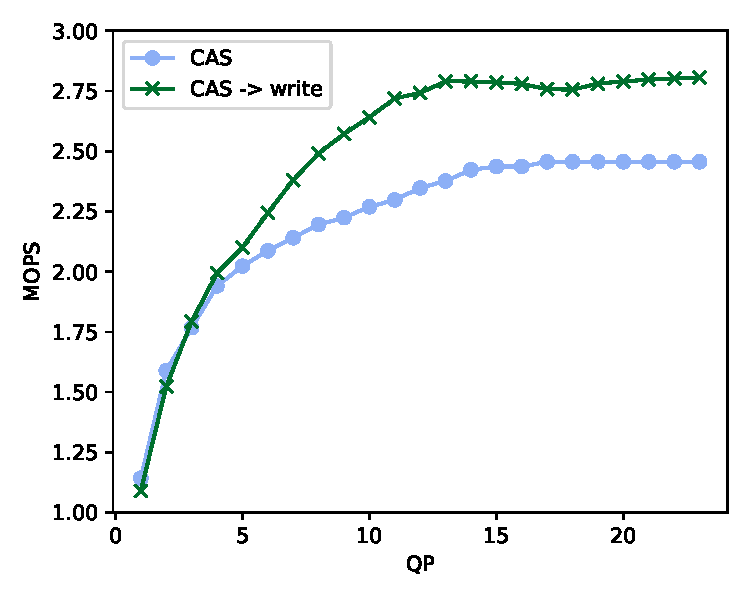
\includegraphics[width=0.5\textwidth]{fig/cas_vs_swap.pdf}
    \caption{Performance Improvement from Swapping CAS to Write on a single key}
    \label{fig:cas_vs_swap}
\end{figure}

We show the raw performance improvement of swapping compare and swap operations
to writes by running an experiment which explicitly tests CAS contention. Each
client core is given a single QP, and all clients make CAS requests to the same
shared location. We measure the performance as the number of clients requesting
the same shared address is increased. All requests are routed through our
middlebox. In the default case, cas operations flow through without
interference. We set the number of cores on our middlebox to 24 so that in our
maximal test case each client thread flows through exactly one middlebox core
for the lowest degree of interference between QP. In our CAS to Write
configuration all client cores request the same address, and as such all are
routed onto the same destination QP. Note that this configuration has the
highest degree of contention for our middlebox as 24 client threads must be
multiplexed to and from a single client connection. Further due to DPDK queue to
core partitioning requirements all TX for a destination QP must be done by a
specific core. Because of this requirement all requests must flow through a
single core prior to being issued to the memory side NIC.

Figure~\ref{fig:cas_vs_swap} Show the performance improvement gained by
converting CAS operations to writes. Both configurations hit distinct
bottlenecks. CAS operations bottleneck due to being applied to a single key. In
the case of converting CAS to write, the bottleneck is the processing power of
our CPU cores. The maximum throughput our prototype can process is 2.8 million
operations per second per core. In this configuration all requests to the memory
server must be processed by the same TX core. As such our bottleneck is
approximately 2.8 MOPS. Hardware implemented CRC, cache tuning, and better lock
management for TX queues could yield higher per core performance in the future.



